\documentclass[multi=tikzpicture,border=7pt]{standalone}
\usepackage{ctex,amsmath,bm}
\usepackage{tikz}
\usetikzlibrary{arrows.meta,calc,angles,quotes,decorations.pathmorphing,patterns}
\tikzset{axis/.style={->,>=Stealth,thick},force/.style={->,>=Stealth,very thick},
flow/.style={->,>=Stealth,thick,blue!70!black},dim/.style={<->,>=Stealth,thin},
body/.style={draw=black,fill=blue!10,thick}}
\begin{document}

% 01 question-01
\begin{tikzpicture}[scale=1]
  \draw[line width=3pt,blue!35!black] (-4,0)--(4,0);
  \filldraw (0,0) circle(2.5pt) node[below]{$O$};
  \filldraw[fill=white] (2,2.6) circle(.14) node[right]{孙鹏，$m/3$};
  \draw[dim] (2.45,.08)--(2.45,2.58) node[midway,right]{$h$};
  \draw[dim] (0,-.45)--(2,-.45) node[midway,below]{$L/4$};
  \draw[flow] (1.65,2.25)--(1.65,1.45) node[midway,left=3pt]{下落};
  \draw[dashed] (-3.464102,2)--(3.464102,-2);

  \draw[->] (2.8,.05) arc[start angle=0,end angle=-30,radius=2.8];
  \node at (3.1,-1.15){$30^\circ$};
\end{tikzpicture}

% 02 solution-01
\begin{tikzpicture}[scale=1]
  \begin{scope}
\draw[dashed] (-2.8,0)--(2.8,0);\draw[line width=3pt,blue!35!black] (-2.81908,1.02606)--(2.81908,-1.02606);
\coordinate (S) at (1.69145,-.615636);\fill (0,0) circle(2pt) node[above left]{$O$};\filldraw[fill=orange!35] (S) circle(.15) node[above right]{孙鹏};
\draw[force] (S)--++(0,-1.3) node[right]{$mg/3$};\draw[dim] (-.15,.5)--(1.54145,-.115636) node[midway,above]{$r$};
\draw[dashed] (S)--(1.69145,-2.3);\draw[dim] (0,-2.2)--(1.69145,-2.2) node[midway,below]{$r\cos\theta$};
\draw[->] (.65,0) arc[start angle=0,end angle=-20,radius=.65];\node at (.95,-.17){$\theta$};
\node at (.5,-3.05){$\tau_O=(mg/3)r\cos\theta$，顺时针};
  \end{scope}
  \begin{scope}[shift={(8,0)},rotate=-30]
    \draw[line width=3pt,blue!35!black] (-3,0)--(3,0);
    \filldraw (0,0) circle(2.5pt) node[below]{$O$};
    \filldraw[fill=orange!35] (2.25,0) circle(.16) node[above]{孙鹏};
    \filldraw[fill=green!35!white] (-1.125,0) circle(.18) node[below]{黄俏};

  \end{scope}
  \draw[force,red!70!black] (7.025721,.5625)--(7.025721,-.8875) node[left]{$(2m/3)v$};
  \node at (8,-2.1){碰撞瞬间对 $O$ 点取角动量矩};
\end{tikzpicture}

% 03 question-02
\begin{tikzpicture}[scale=.9]
\draw[fill=blue!8,thick] (0,0) circle(1);\node at (0,0){地球};
\draw[dashed,blue!70!black,thick] (-1.8962507,0) ellipse[x radius=3.1869401,y radius=2.5614098];
\coordinate (P) at (0.0985840,1.9975688);\fill (P) circle(3pt) node[above right]{飞船};
\draw[thick] (0,0)--(P) node[midway,right]{$r_0=2R_E$};
\draw[dashed] (P)--++(0.0492920,0.9987844);
\draw[flow] (P)--++(-1.2184737,0.7860165) node[left]{$\boldsymbol v_0$};
\draw[->] ($(P)+(87.1746301:.65)$) arc[start angle=87.1746301,end angle=147.1746301,radius=.65];
\node at ($(P)+(117.1746301:.95)$){$60^\circ$};
\node[align=center] at (-2,-3.7){以 $R_E$ 为长度单位；地心为焦点\\箭头沿轨道切线，选径向外行的状态};
\end{tikzpicture}

% 04 solution-02
\begin{tikzpicture}[x=1cm,y=10cm]
\draw[axis] (.8,0)--(6,0) node[right]{$u=r/R_E$};\draw[axis] (1,-.23)--(1,.1) node[above]{$\widetilde U$};
\draw[blue!70!black,very thick,domain=1:5.7,samples=160] plot(\x,{1.029329085/(\x*\x)-1/\x});
\draw[red!70!black,thick] (1,-0.156890305)--(5.7,-0.156890305) node[right]{$\widetilde\varepsilon$};
\foreach \x/\lab in {1.290689349/r_p,5.083190802/r_a}{\draw[dashed] (\x,0)--(\x,-0.156890305);\fill[red!70!black] (\x,-0.156890305) circle(2pt);\node[above] at (\x,0){$\lab$};}
\node at (3.2,-.29){曲线 $h_s^2/(2\mu R_Eu^2)-1/u$；交点为实际近、远地点};
\end{tikzpicture}

% 05 question-03
\begin{tikzpicture}
  \fill[orange!18] (-4,0) circle(1.25); \draw[thick] (-4,0) circle(1.25);
  \fill[blue!18] (3.5,0) circle(.7); \draw[thick] (3.5,0) circle(.7);
  \draw[thick] (-2.75,0)--(2.8,0);
  \draw[dim] (-4,-1.65)--(3.5,-1.65) node[midway,below]{$r_0$};
  \draw[dashed] (3.5,0) circle(1.55);
  \draw[dim] (3.5,.2)--(5.05,.2) node[midway,above]{$R_h$};
  \node at (-4,0){恒星 $M_0$}; \node at (3.5,0){行星 $M$};
  \filldraw (5.05,0) circle(.09) node[right]{卫星};
\end{tikzpicture}

% 06 solution-03
\begin{tikzpicture}
  \fill[orange!18] (-4,0) circle(1.1); \draw[thick] (-4,0) circle(1.1);
  \fill[blue!18] (3.2,0) circle(.6); \draw[thick] (3.2,0) circle(.6);
  \node[below] at (3.2,-.65){行星};
  \draw[dashed,blue!65!black,thick] (3.2,0) circle(2.05);
  \node[blue!65!black] at (3.2,2.35){希尔球边界 $R_h$};
  \filldraw (5.25,0) circle(.08) node[above right]{试探卫星};
  \draw[force,red!70!black] (5.15,.22)--(3.85,.22);
  \node[red!70!black] at (4.65,1.05){行星引力 $GMm/r^2$};
  \draw[force,blue!70!black] (5.35,-.25)--(6.75,-.25)
    node[midway,below]{引力梯度＋离心差力};
  \draw[dim] (3.2,-1.15)--(5.25,-1.15) node[midway,below]{$r$};
  \node at (.2,-1.7){希尔球边界：行星引力与共转系差力同量级};
\end{tikzpicture}

% 07 question-04
\begin{tikzpicture}
  \draw[axis] (-1,0)--(5.2,0) node[right]{$x$};
  \draw[axis] (0,-2.5)--(0,3.2) node[above]{$y$};
  \draw[line width=3pt,blue!50!black] (-3.1,0)--(3.1,0);
  \filldraw[fill=red!25] (3.1,0) circle(.14) node[above]{$+q$};
  \filldraw[fill=blue!25] (-3.1,0) circle(.14) node[above]{$-q$};
  \draw[flow,orange!90!black] (.4,2.4)--(3.1,2.4) node[right]{$\bm E_0$};
  \node at (3.6,-1.5){$\otimes\,\bm B_0$};
  \draw[flow] (0,.25)--(0,1.65) node[right]{$v_0$};
  \draw[dashed,blue!70!black,thick] (-3.05298,-.53831)--(3.05298,.53831);
  \node[above] at (-2,0){水平参考位置};
  \coordinate (Xo) at (3.1,0); \coordinate (Oo) at (0,0); \coordinate (Ro) at (3.05298,.53831);
  \draw pic[draw,->,"$\theta_0$",angle radius=1.15cm,angle eccentricity=1.25]{angle=Xo--Oo--Ro};
\end{tikzpicture}

% 08 solution-04
\begin{tikzpicture}
\draw[axis] (-4.5,0)--(4.6,0) node[right]{$x$};\draw[axis] (0,-1.8)--(0,3.3) node[above]{$y$};
\draw[line width=3pt,blue!50!black] (-2.934443,-.623735)--(2.934443,.623735);
\filldraw[fill=red!25] (2.934443,.623735) circle(.13) node[right=5pt]{$+q$};\filldraw[fill=blue!25] (-2.934443,-.623735) circle(.13) node[left=5pt]{$-q$};
\draw[force,orange!85!black] (2.934443,1.2)--++(1.05,0) node[right]{$qE_0$};\draw[force,orange!85!black] (-2.934443,-1.2)--++(-1.05,0) node[left]{$qE_0$};
\draw[force,purple!75!black] (2.934443,.4)--++(-1.05,0) node[midway,below=6pt]{$qB_0v_0$};\draw[force,purple!75!black] (-2.934443,-.4)--++(1.05,0) node[midway,above=6pt]{$qB_0v_0$};
\draw[flow] (.2,1)--(.2,2.5) node[right]{$v_0$};\node at (3,-1.3){$\otimes\,\boldsymbol B_0$};
\node[align=center] at (0,-2.15){图取 $t=0$、$\dot\theta=0$，两端速度都沿 $+y$\\磁力水平相反；力箭头略作平移以免重叠};\end{tikzpicture}

% 09 question-05
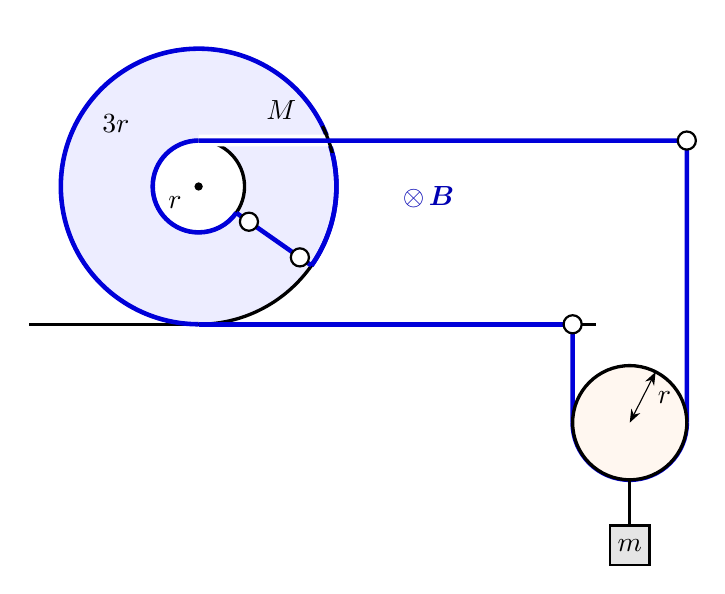
\begin{tikzpicture}[x=1cm,y=1cm]
  \tikzset{wire/.style={draw=blue!85!black,line width=1.65pt}}

  % 复合圆盘及桌面
  \coordinate (C) at (-2.2,1.75);
  \def\Rout{1.75}
  \def\Rin{.583333333}
  \draw[very thick] (-4.35,0)--(2.85,0);
  \draw[very thick,fill=blue!7] (C) circle(\Rout);
  \draw[very thick,fill=white] (C) circle(\Rin);
  \fill (C) circle(1.5pt);
  \node at (-1.15,2.72){$M$};
  \node at (-2.50,1.54){$r$};
  \node at (-3.25,2.55){$3r$};

  % 单根导线在复合圆盘上的连续路径：
  % 内圆盘上切点 -> 内圆盘长绕段 -> 径向段 r 到 3r
  % -> 外圆盘长绕段 -> 外圆盘下切点。
  \coordinate (InnerTop) at ($(C)+(90:\Rin)$);
  \coordinate (InnerRadial) at ($(C)+(-35:\Rin)$);
  \coordinate (OuterRadial) at ($(C)+(-35:\Rout)$);
  \coordinate (OuterBottom) at ($(C)+(-90:\Rout)$);
  \draw[wire] (InnerTop) arc[start angle=90,end angle=325,radius=\Rin];
  \draw[wire] (InnerRadial)--(OuterRadial);
  \draw[wire] (OuterRadial) arc[start angle=-35,end angle=270,radius=\Rout];

  % 固定在大圆盘右下方、沿同一半径排列的两个轻滑轮。
  \coordinate (DiskPulleyInner) at ($(C)+(-35:.78)$);
  \coordinate (DiskPulleyOuter) at ($(C)+(-35:1.57)$);
  \filldraw[fill=white,thick] (DiskPulleyInner) circle(.115);
  \filldraw[fill=white,thick] (DiskPulleyOuter) circle(.115);

  % 两个定滑轮与半径为 r 的动滑轮。
  \coordinate (UpperFixed) at (4.00,2.333333333);
  \coordinate (LowerFixed) at (2.55,0);
  \coordinate (MovingCenter) at (3.275,-1.25);
  \def\Rmoving{.725}

  % 上方直线跨过外圆盘绕段但不与之连接；白色衬线表示跨线。
  \draw[white,line width=4.2pt] (InnerTop)--(UpperFixed);
  \draw[very thick] ($(C)+(14:\Rout)$)
    arc[start angle=14,end angle=26,radius=\Rout];
  \draw[wire] (OuterRadial)
    arc[start angle=-35,end angle=14,radius=\Rout];
  \draw[wire] (InnerTop)--(UpperFixed);
  \draw[wire] (UpperFixed)--($(MovingCenter)+(0:\Rmoving)$);
  \draw[wire] ($(MovingCenter)+(0:\Rmoving)$)
    arc[start angle=0,end angle=-180,radius=\Rmoving];
  \draw[wire] ($(MovingCenter)+(180:\Rmoving)$)--(LowerFixed);
  \draw[wire] (LowerFixed)--(OuterBottom);

  \filldraw[fill=white,thick] (UpperFixed) circle(.115);
  \filldraw[fill=white,thick] (LowerFixed) circle(.115);
  \draw[very thick,fill=orange!6] (MovingCenter) circle(\Rmoving);
  \draw[dim] (MovingCenter)--++(63:\Rmoving)
    node[midway,right=2pt]{$r$};

  % 动滑轮下方用绝缘绳悬挂重物。
  \draw[very thick] ($(MovingCenter)+(0,-\Rmoving)$)--++(0,-.58);
  \draw[fill=gray!20,thick]
    ($(MovingCenter)+(-.25,-1.305)$) rectangle
    ($(MovingCenter)+(.25,-1.805)$) node[midway]{$m$};

  \node[blue!70!black] at (.72,1.62){$\otimes\,\bm B$};
\end{tikzpicture}

% 10 solution-05
\begin{tikzpicture}[x=.78cm,y=.78cm]
  \begin{scope}[shift={(-5.2,0)}]
    \node[font=\bfseries] at (1.7,4.25){(a) 切点速度与绳长约束};
    \coordinate (C) at (0,1.75);
    \coordinate (A) at (0,2.333333333);
    \coordinate (D) at (0,0);
    \draw[very thick] (-2.15,0)--(2.1,0);
    \draw[very thick,fill=blue!7] (C) circle(1.75);
    \draw[very thick,fill=white] (C) circle(.583333333);
    \fill (C) circle(1.5pt) node[left=3pt]{$C$};
    \filldraw[fill=white,thick] (A) circle(.10) node[left=4pt]{$A$};
    \filldraw[fill=white,thick] (D) circle(.10) node[below left]{$D$};
    \draw[flow] (-.35,1.75)--(1.20,1.75) node[midway,above]{$V_C$};
    \draw[flow,purple!75!black] (1.95,1.75)
      arc[start angle=0,end angle=-72,radius=.78] node[right]{$\omega$};
    \draw[flow,blue!70!black] (.18,2.333333333)--(1.72,2.333333333)
      node[midway,above=5pt]{$u_A=V_C+r\omega$};
    \node[blue!70!black,anchor=west] at (.18,.34){$u_D=V_C-3r\omega=0$};

    \coordinate (P) at (3.55,-.55);
    \draw[blue!75!black,very thick] (A)--(2.9,2.333333333)--(2.9,-.55);
    \draw[blue!75!black,very thick] (D)--(4.20,0)--(4.20,-.55);
    \draw[very thick,fill=orange!7] (P) circle(.65);
    \draw[blue!75!black,very thick]
      ($(P)+(180:.65)$) arc[start angle=180,end angle=360,radius=.65];
    \draw[flow,red!70!black] (3.55,-1.25)--(3.55,-2.333333333)
      node[right]{$v_0$};
    \node[draw,rounded corners,fill=blue!5,align=center,font=\small]
      at (1.55,-2.55)
      {$V_C=3r\omega$\\
       $2v_0-u_A-u_D=0$\\
       $\Rightarrow\ V_C=\dfrac32v_0$};
  \end{scope}

  \begin{scope}[shift={(5.0,0)}]
    \node[font=\bfseries] at (0,4.25){(b) 三段运动电动势逐项列账};
    \node[draw,rounded corners,fill=green!6,align=left,text width=8.1cm,
      inner sep=8pt] at (0,1.70)
      {\textcolor{blue!75!black}{动滑轮直径等效段：}
       $\mathcal E_1=+B(2r)v_0$\\[5pt]
       \textcolor{purple!75!black}{圆盘径向转动段：}
       $\mathcal E_2=+\displaystyle\int_r^{3r}B\omega s\,ds
       =+4B\omega r^2$\\[5pt]
       \textcolor{red!70!black}{圆盘平动等效段：}
       $\mathcal E_3=-B(4r)V_C$\\[7pt]
       $\mathcal E=\mathcal E_1+\mathcal E_2+\mathcal E_3
       =-2Brv_0$};
    \node[draw,rounded corners,fill=orange!8,align=center]
      at (0,-1.55)
      {$mgv_0\ \longrightarrow\ |\mathcal E|I
       \ \longrightarrow\ I^2R$\\
       $mgv_0=\dfrac{\mathcal E^2}{R}$};
    \draw[force] (-2.7,-2.65)--(-2.7,-3.55) node[right]{$mg$};
    \draw[force,green!45!black] (2.7,-3.45)--(2.7,-2.55)
      node[right]{等效电磁阻力};
  \end{scope}
\end{tikzpicture}

% 11 question-06
\begin{tikzpicture}
\draw[axis] (-.2,0)--(7.4,0) node[right]{$E$};\draw[axis] (0,-.2)--(0,5.2) node[above]{$T$};
\coordinate (A) at (5.8,4.3);\coordinate (B) at (1.1,4.3);\coordinate (C) at (1.1,1.2);\coordinate (D) at (5.8,1.2);
\draw[flow] (A)--(B) node[midway,above]{1：等温 $T_1$};\draw[flow] (B)--(C) node[midway,left]{2：$E_2$};\draw[flow] (C)--(D) node[midway,below]{3：等温 $T_2$};\draw[flow] (D)--(A) node[midway,right]{4：$E_1$};
\node[above right] at (A){$(E_1,T_1)$};\node[above left] at (B){$(E_2,T_1)$};\node[below left] at (C){$(E_2,T_2)$};\node[below right] at (D){$(E_1,T_2)$};\end{tikzpicture}

% 12 solution-06
\begin{tikzpicture}
\draw[axis] (-.2,0)--(7.2,0) node[right]{$E$};\draw[axis] (0,-.2)--(0,5.2) node[above]{$P$};
\draw[blue!70!black,thick] (0,0)--(6.3,4.2) node[right]{$P=\chi(T_1)E$};\draw[red!70!black,thick] (0,0)--(6.3,3.0) node[right]{$P=\chi(T_2)E$};
\fill[orange!25] (1.4,.933333)--(5.3,3.533333)--(5.3,2.523810)--(1.4,.666667)--cycle;
\draw[flow] (5.3,3.533333)--(1.4,.933333);\draw[flow] (1.4,.933333)--(1.4,.666667);\draw[flow] (1.4,.666667)--(5.3,2.523810);\draw[flow] (5.3,2.523810)--(5.3,3.533333);
\draw[dashed] (1.4,0)--(1.4,.666667) node[below]{$E_2$};\draw[dashed] (5.3,0)--(5.3,2.523810) node[below]{$E_1$};
\node at (3.5,-.8){阴影面积乘 $V$ 为净输出功，取 $\alpha>0$};\end{tikzpicture}

% 13 question-07
\begin{tikzpicture}
\draw[fill=blue!8,thick] (0,-1.8) rectangle (2,1.8);\node at (1,1.25){玻璃 $n$};\node at (-2,1.25){空气};\node at (4,1.25){空气};
\draw[flow] (-3,0)--(0,0) node[midway,below]{$u_0$};\draw[flow,red!70!black] (0,.3)--(-2,.3) node[midway,above]{反射};\draw[flow,green!45!black] (2,0)--(4.5,0) node[midway,below]{透射};
\draw[dim] (0,-2.15)--(2,-2.15) node[midway,below]{$a$};\end{tikzpicture}

% 14 solution-07
\begin{tikzpicture}
\fill[blue!5] (0,-2.4) rectangle (4,2.4);\draw[very thick] (0,-2.4)--(0,2.4) (4,-2.4)--(4,2.4);
\node[above] at (0,2.4){前界面};\node[above] at (4,2.4){后界面};
\draw[flow] (-2,2.2)--(0,2) node[midway,above=7pt]{$u_0$};\draw[flow,red!70!black] (0,2)--(-2,1.8) node[midway,above]{$ru_0$};
\draw[flow] (0,2)--(4,1)--(0,0)--(4,-1)--(0,-2);\draw[flow,purple!70!black] (0,-2)--(-2,-2.2) node[left]{$tt'r'^3e^{2i\delta}u_0$};
\node[right] at (0,2){$t$};\foreach \x/\y in {4/1,0/0,4/-1}{\fill (\x,\y) circle(2pt);\node[above right] at (\x,\y){$r'$};}\node[right] at (0,-2){$t'$};
\foreach \y in {1.5,.5,-.5,-1.5}{\node[fill=white,inner sep=1pt] at (2,\y){$e^{i\delta/2}$};}
\draw[dashed,flow] (0,0)--(-1.5,-.15);\draw[dashed,flow] (4,1)--(5.5,.85);\draw[dashed,flow] (4,-1)--(5.5,-1.15);
\node[align=center] at (2,-3.15){法向光路上下错开以便计数；四个单程、三次内部反射\\$\delta=4\pi na/\lambda_0$ 为一次往返相位};\end{tikzpicture}

% 15 question-08
\begin{tikzpicture}[scale=.9]
  \begin{scope}
    \draw[axis] (-.3,0)--(3.5,0) node[right]{$x$}; \draw[axis] (0,-.2)--(0,4) node[above]{$y$};
    \draw[very thick] (-1.3,.4)--(-1.3,3.2); \node[left] at (-1.3,3.2){$A$}; \node[left] at (-1.3,.4){$B$};
    \draw[flow] (-1.6,3.6)--(-.3,3.6) node[midway,above]{$\beta c$};
    \draw[dashed] (0,0)--(0,-1.25); \draw[fill=gray!25] (-.25,-1.55) rectangle (.25,-1.25);
  \end{scope}
  \begin{scope}[shift={(6,0)}]
    \draw[axis] (-.3,0)--(3.5,0) node[right]{$x$}; \draw[axis] (0,-.2)--(0,4) node[above]{$y$};
    \draw[very thick] (-1.33,.4) rectangle (.83,3.1);
    \node at (-1.35,2.85){$A$}; \node at (-1.35,.65){$B$}; \node at (.85,.65){$C$}; \node at (.85,2.85){$D$};
    \draw[flow] (-1.6,3.55)--(-.3,3.55) node[midway,above]{$\beta c$};
    \draw[dashed] (0,0)--(0,-1.25); \draw[fill=gray!25] (-.25,-1.55) rectangle (.25,-1.25);
  \end{scope}
  \begin{scope}[shift={(12,0)}]
    \draw[axis] (-.3,0)--(3.5,0) node[right]{$x$}; \draw[axis] (0,-.2)--(0,4) node[above]{$y$};
    \draw[very thick] (-.5,1.75) ellipse[x radius=1.08,y radius=1.35]; \node at (-.5,1.75){$r$};
    \draw[flow] (-1.6,3.55)--(-.3,3.55) node[midway,above]{$\beta c$};
    \draw[dashed] (0,0)--(0,-1.25); \draw[fill=gray!25] (-.25,-1.55) rectangle (.25,-1.25);
  \end{scope}
\node[align=center] at (6,-2.3){地面系同一时刻的位置图（$\beta=0.6$），不是照片\\中图为立方体 $xy$ 截面；未画出的 $z$ 向棱长仍为 $l$};\end{tikzpicture}

% 16 solution-08
\begin{tikzpicture}
\begin{scope}
\draw[fill=blue!7,very thick] (0,0) rectangle (4.2,3);\draw[thick] (1.8,0)--(1.8,3);
\node at (.9,1.5){侧面};\node at (3,1.5){正面};\draw[dim] (0,-.45)--(1.8,-.45) node[midway,below]{$\beta l=0.6l$};\draw[dim] (1.8,-.95)--(4.2,-.95) node[midway,below]{$l/\gamma=0.8l$};\draw[dim] (-.4,0)--(-.4,3) node[midway,left]{$l$};\node at (2.1,3.5){(a) 立方体的远场照片};
\end{scope}
\begin{scope}[shift={(8,1.5)}]
\draw[very thick] (0,0) circle(2);\draw[axis] (-2.6,0)--(2.8,0) node[right]{$x'$};\draw[axis] (0,-2.6)--(0,2.8) node[above]{$y'$};
\draw[thick] (-1.6,1.2)--(1.6,-1.2);\fill (1.6,-1.2) circle(2pt) node[right]{$R:(0.8r,-0.6r)$};\fill (-1.6,1.2) circle(2pt) node[left]{$L$};
\draw[->] (.7,0) arc[start angle=0,end angle=-36.869898,radius=.7];\node at (1,-.3){$\theta_R$};
\draw[->] (1.1,0) arc[start angle=0,end angle=143.130102,radius=1.1];\node at (.1,1.4){$\theta_L$};
\node[align=center] at (0,-3.2){(b) 共动系 $z'=0$ 截面\\$\theta_R=-\arcsin\beta$，$\theta_L=\pi-\arcsin\beta$};
\end{scope}\end{tikzpicture}

\end{document}
